Los asistentes de demostración son herramientas que facilitan la escritura y chequeo de demostraciones en una computadora. Se pueden usar para formalizar teoremas y realizar verificación formal de programas, entre otros. A diferencia de escribir demostraciones y chequearlas manualmente, el uso de asistentes permite la colaboración a gran escala: no es necesario confiar ni revisar a detalle las demostraciones que hace el resto del equipo, alcanza con que el asistente las considere válidas. También facilitan la generación de demostraciones con técnicas de inteligencia articial, que muchas veces usan razonamientos lógicos erróneos difíciles de detectar a mano. Pero se puede delegar su verificación al asistente.

Trabajan con distintas \textit{teorías}. Por ejemplo, el asistente Mizar \cite{mizar} con lógica de primer orden, Coq \cite{coq} con teoría de tipos (cálculo de construcciones o CoC) y Agda \cite{agda} también (teoría unificada de tipos dependientes, basada en teoría de tipos de Martin-Löf).

Una propiedad deseable cumplida por muchos asistentes es el \textbf{criterio de De Bruijn} \cite{freek-bruijn}. En principio, para estar seguros de que una demostración es correcta sería necesario confiar en la implementación del asistente, que puede ser muy compleja. Un asistente se dice que cumple con el criterio si construye una demostración en un formato elemental, sencillo, que pueda ser chequeada por un programa independiente, escrito por cualquiera que desconfíe de la implementación original del asistente.

En este trabajo diseñamos e implementamos un asistente de demostración \textit{PPA}
(\textit{Pani's proof assistant}). Trabaja sobre teorías de lógica clásica de
primer orden. Cumple con el criterio de De Bruijn porque \textit{certifica} las
demostraciones en el lenguaje de alto nivel \ppaLang{}, generando demostraciones
de bajo nivel en el sistema de deducción natural de Gentzen \cite{gentzen-1935}. Su sintaxis está inspirada en el
\textit{mathematical vernacular} introducido por Freek Wiedijk
\cite{freek-mv} \cite{wenzel-isar}, que tiene por objetivo ser lo más parecido posible al lenguaje
natural. No es un demostrador automático de teoremas, pero su mecanismo de
demostración principal, el \textbf{by}, incluye un pequeño demostrador
heurístico para lógica de primer orden y completo para proposicional, que
simplifica la escritura de demostraciones. Está inspirado en el mecanismo análogo de Mizar \cite{freek-by}.

Algunos asistentes de demostración implementan la \textit{extracción de testigos
de existenciales}. Dada una demostración de $\exists \var . \pred(\var)$,
encuentran un \textit{testigo} $\term$ tal que cumpla $\pred(\term)$. Para ello,
es deseable que las demostraciones sean \textbf{constructivas}: una demostración
de $\exists \var . \pred(\var)$ nos debe decir cómo encontrar a un objeto
$\term$ que cumpla con $\pred(\term)$. PPA usa lógica clásica, que no siempre es constructiva por sus principios de razonamiento clásicos. Por ejemplo, con el principio del tercero excluido o LEM (\textit{law of excluded middle}), siempre
vale $\form \fOr \fNot \form$, y podemos realizar una demostración que al usarlo no explicite cual de las dos es la que vale. Los asistentes como Coq
aseguran el constructivismo mediante el uso de \textbf{lógica intuicionista},
que siempre es constructiva por su naturaleza.

En general se pueden encontrar dos grandes categorías de extracción de testigos para lógica clásica. Las \textbf{directas}, mediante semánticas operacionales de cálculos $\lambda$ clásicos, como \textit{realizabilidad clásica} \cite{miquel-friedman}, y las \textbf{indirectas}, que traducen las demostraciones a otra lógica, como la intuicionista.

En este trabajo, la extracción se hace de forma \textit{indirecta} en dos pasos.
Primero hacemos uso de la \textbf{traducción de Friedman}
\cite{selinger-friedman}, que permite traducir una demostración clásica a una
intuicionista para cierta clase de fórmulas: las $\classPiTwo$, de la forma
$\forall \var_1 \dots \forall \var_n . \exists \varTwo . \anyForm$. Luego,
\textit{normalizamos} la demostración intuicionista, y de su forma normal
extraemos el testigo del existencial. Hasta donde sabemos, no hay asistentes de demostración para lógica clásica que implementen la extracción de testigos basándose en estas técnicas. Este es el aporte principal del trabajo.

\section{Lógica de primer orden}

A continuación se presentan definiciones preliminares de lógica de primer orden. Suponemos dados:

\begin{itemize}
    \item Un conjunto infinito numerable de \textbf{variables}
    \(
        \{\var, \varTwo, \varThree, \dots\}.
    \)
    \item Un conjunto infinito numerable de \textbf{símbolos de función}
    \(
        \{\fun, \funTwo, \funThree, \dots\}.
    \)
    \item Un conjunto infinito numerable de \textbf{símbolos de predicado}
    \(
        \{\pred, \predTwo, \predThree, \dots\}.
    \)
\end{itemize}

\begin{definition}[Términos]
    Los términos están dados por la gramática
    \begin{align*}
        \term ::= &\ \var                               &\text{(variables)} \\
                  & \mid \fun(\term_1, \dots, \term_n) &\text{(funciones)}
    \end{align*}
\end{definition}

\begin{definition}[Fórmulas]
    Las fórmulas están dadas por la gramática
    \begin{align*}
        \form, \formTwo ::=
         & \ \pred(\term_1, \dots, \term_n) & (\text{predicados})                \\
         & \mid \fFalse                     & \text{(falso o \textit{bottom})}         \\
         & \mid \fTrue                      & \text{(verdadero o \textit{top})} \\
         & \mid \form \fAnd \formTwo        & \text{(conjunción)}                \\
         & \mid \form \fOr \formTwo         & \text{(disyunción)}                \\
         & \mid \form \fImp \formTwo        & \text{(implicación)}               \\
         & \mid \fNot \form                 & \text{(negación)}                  \\
         & \mid \forall \var . \form        & \text{(cuantificador universal)}   \\
         & \mid \exists \var . \form        & \text{(cuantificador existencial)}
    \end{align*}

    Los predicados son \textbf{fórmulas atómicas}. Los de aridad 0 además son llamados \textit{variables proposicionales}.
\end{definition}

\begin{notation*}
    Usamos
    \begin{itemize}
        \item $\formLit, \formLitTwo, \formLitThree, \dots$, $\form, \formTwo, \formThree, \dots$ y $\anyForm, \anyFormTwo, \dots$ para referirnos a fórmulas.
        \item $\term, \termTwo, \dots$ para referirnos a términos
    \end{itemize}
\end{notation*}

\begin{definition}[Variables libres y ligadas]
    Las variables pueden ocurrir libres o ligadas. Los cuantificadores son los que las ligan. El conjunto de variables libres de un término o fórmula $X$ se nota $\fv{X}$ y se define recursivamente de la siguiente manera.

    \begin{itemize}
        \item Términos
        \begin{align*}
            \fv{\var} &= \{ \var \}\\
            \fv{\fun(\term_1, \dots, \term_n)} &= \bigcup_{i \in 1\dots n} \fv{t_i} 
        \end{align*}
    
        \item Fórmulas
        \begin{align*}
            \fv{\fFalse} &=\emptyset\\
            \fv{\fTrue} &=\emptyset \\
            \fv{\pred(\term_1, \dots, \term_n)} &= \bigcup_{i \in 1\dots n} \fv{t_i} \\
            \fv{\form \fAnd \formTwo} &= \fv{\form} \cup \fv{\formTwo}\\
            \fv{\form \fOr \formTwo} &=\fv{\form} \cup \fv{\formTwo}\\
            \fv{\form \fImp \formTwo} &=\fv{\form} \cup \fv{\formTwo}\\
            \fv{\fNot \form} &=\fv{\form}\\
            \fv{\forall \var . \form} &= \fv{\form} \setminus \var \\
            \fv{\exists \var . \form} &= \fv{\form} \setminus \var
        \end{align*}
    \end{itemize}
\end{definition}


\section{Arquitectura de \ppaTool{}}

A lo largo del trabajo, usaremos la sigla ``PPA'' para referirnos a dos cosas separadas: \ppaLang{} el lenguaje para escribir demostraciones, y \ppaTool{} la herramienta que implementa el lenguaje y la extracción de testigos,  implementada en \textbf{Haskell}. Funcionalmente tiene la siguiente arquitectura representada gráficamente en la \fullref{intro:fig:ppa-arch}.

\begin{itemize}
    \item El usuario escribe una demostración en alto nivel en el lenguaje \ppaLang{}.
    \item Puede \textit{chequear} la demostración de alto nivel, que primero se \textbf{certifica} generando una demostración en deducción natural de bajo nivel (el ``certificado''), para que luego un módulo independiente chequee su correctitud.
    Si el usuario escribe una demostración inválida, debería fallar el certificador y reportar un error al usuario. De todas formas, el certificado es verificado por el chequeador de deducción natural como mecanismo de \textit{fallback}.
    \item Si es una demostración de un existencial, el usuario puede optar por \textit{extraer un testigo}: primero se \textbf{traduce} la demostración de clásica a intuicionista, y luego se reduce hacia su formal normal de la cual se puede tomar el testigo.
\end{itemize}

Describimos los tipos de las principales funciones que implementan las distintas etapas de la herramienta.

\begin{itemize}
    \item El tipo \mintinline{haskell}{type Result a = Either String a} es la mónada principal que se usa para devolver resultados o errores.
    \item \mintinline{haskell}{certify :: Program -> Result Context}. Implementada por el módulo \texttt{PPA.Certifier}. Donde \mintinline{haskell}{Program} es el tipo de los programas escritos en PPA (listas de axiomas y teoremas) y \mintinline{haskell}{Context} el tipo de los certificados (lista de axiomas y teoremas junto con su demostración en deducción natural).
    \item \mintinline{haskell}{check :: Env -> Proof -> Form -> CheckResult}.
    Implementada por el módulo \texttt{ND.Checker}. Chequea una demostración de una fórmula asumiendo un entorno o contexto de demostración. El tipo \mintinline{haskell}{Env} representa los contextos en deducción natural (asociación de etiquetas a fórmulas), \mintinline{haskell}{Proof} las demostraciones en deducción natural, \mintinline{haskell}{Form} las fórmulas de primer orden y \mintinline{haskell}{CheckResult} es una sofisticación de \mintinline{haskell}{Result} específica para el chequeo.
    \item \mintinline{haskell}{translateFriedman :: Proof -> FormPi02 -> (Proof, R)}. Implementada por el módulo \texttt{Extractor.Translator.Proof}. Traduce una demostración clásica de una fórmula $\classPiTwo$ generando una demostración intuicionista, usando la traducción de Friedman parametrizada por una fórmula \mintinline{haskell}{R}. Esta parametrización se explicará en detalle más adelante, en el \namedref{chap:witness-extraction}. El tipo \mintinline{haskell}{FormPi02} es un refinamiento del de las fórmulas, \mintinline{haskell}{Form}, que solo representa las de la clase $\classPiTwo$.
    \item \mintinline{haskell}{reduce :: Proof -> Proof}. Reduce una demostración a su forma normal. Implementada en el módulo \texttt{Extractor.Reducer}.
\end{itemize}

\begin{figure}[h]
    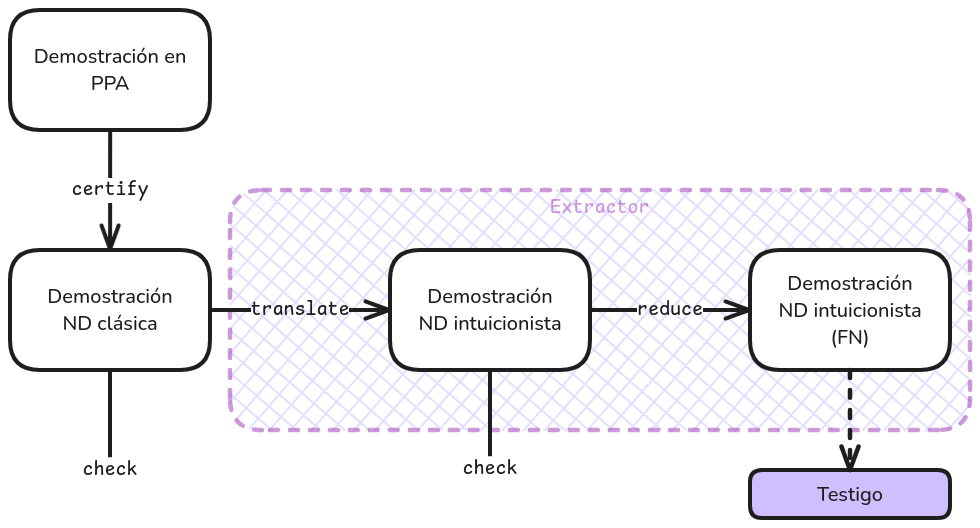
\includegraphics[scale=0.42]{img/arch.png}
    \centering
    \caption{Representación gráfica de la arquitectura funcional de \ppaTool{}}
    \medskip
    \small
    Cada caja corresponde a las versiones de una demostración durante el flujo del programa, y las flechas están etiquetadas por la función que realiza la transformación. Primero es representada en el lenguaje de alto nivel \ppaLang{}, transformada mediante \mintinline{haskell}{certify} al sistema de deducción natural (ND) clásico, traducida a intuicionista por \mintinline{haskell}{translateFriedman} y finalmente reducida a su forma normal (FN) por \mintinline{haskell}{reduce}, a partir de la cual se puede extraer un testigo.
    Además, se representa el mecanismo de \textit{fallback} que verifica la correctitud de cada demostración de deducción natural con \mintinline{haskell}{check}, que permite encontrar problemas en las transformaciones.
    \label{intro:fig:ppa-arch}
\end{figure}

\section{Estructura del escrito}

El trabajo se divide en 5 capítulos principales además de la introducción y la conclusión. Comenzamos por el \fullref{chap:nd} en el que se presenta de forma completa el sistema de deducción natural usado para los certificados. Se introducen las reglas de inferencia junto con sus intuiciones, el concepto de \textit{reglas admisibles}, demostraciones de ejemplo y algunos algoritmos implementados: chequeo (función \mintinline{haskell}{check}), alfa equivalencia de fórmulas y sustitución sin capturas.

En el \fullref{chap:ppa} introducimos el lenguaje desde el punto de vista de un usuario: cómo están compuestos los programas, cómo usar el pequeño demostrador (\lstinline{by}) para facilitar la escritura de demostraciones, y una descripción exhaustiva de todos los comandos soportados. En \fullref{chap:ppa-certifier} se muestra la implementación interna del \textit{certificador} de PPA, cómo genera demostraciones en deducción natural a partir de programas (la función \mintinline{haskell}{certify}). De forma central se explica el funcionamiento del \lstinline{by}, que es el corazón del certificador.

En el \fullref{chap:witness-extraction} se muestra el proceso completo de extracción de testigos, comenzando por la traducción de Friedman y luego la normalización de demostraciones intuicionistas (\mintinline{haskell}{translateFriedman} y \mintinline{haskell}{reduce}).

Finalmente, en el \fullref{chap:ppa-tool} se detallan los pasos para instalar y usar la herramienta \ppaTool{}, y se mencionan algunos detalles de implementación como la arquitectura del programa a nivel módulos y dependencias entre ellos, el compilador y el modelado de deducción natural.